%%%%%%%%%%%%%%%%%%%%%%%%%%%%%%%%%%%%%%%%%%%%%%%%%%%%%%%%%%%%%%%%%%%%%%%%%%%%
% AGUJournalTemplate.tex: this template file is for articles formatted with LaTeX
%
% This file includes commands and instructions
% given in the order necessary to produce a final output that will
% satisfy AGU requirements, including customized APA reference formatting.
%
% You may copy this file and give it your
% article name, and enter your text.
%
%
% Step 1: Set the \documentclass
%
% There are two options for article format:
%
% PLEASE USE THE DRAFT OPTION TO SUBMIT YOUR PAPERS.
% The draft option produces double spaced output.
%

%% To submit your paper:
\documentclass[draft]{agujournal2019}
\usepackage{url} %this package should fix any errors with URLs in refs.
\usepackage{lineno}
\usepackage{color}
\graphicspath{ {figures/} }
\linenumbers
%%%%%%%
% As of 2018 we recommend use of the TrackChanges package to mark revisions.
% The trackchanges package adds five new LaTeX commands:
%
%  \note[editor]{The note}
%  \annote[editor]{Text to annotate}{The note}
%  \add[editor]{Text to add}
%  \remove[editor]{Text to remove}
%  \change[editor]{Text to remove}{Text to add}
%
% complete documentation is here: http://trackchanges.sourceforge.net/
%%%%%%%

\draftfalse

\journalname{JGR: Space Physics}


\begin{document}

\title{Statistical Properties of Curtain Electron Precipitation Derived with AeroCube-6}

%% ------------------------------------------------------------------------ %%
%
%  AUTHORS AND AFFILIATIONS
%
%% ------------------------------------------------------------------------ %%

\authors{M. Shumko\affil{1}, A.T. Johnson\affil{1}, J.G. Sample\affil{1}, D.L. Turner\affil{3}, T.P. O'Brien\affil{2}, and J.B. Blake\affil{2}}


\affiliation{1}{Department of Physics, Montana State University, Bozeman, Montana, USA}
\affiliation{2}{Space Science Applications Laboratory, The Aerospace Corportation, El Segundo, California USA}
\affiliation{3}{Johns Hopkins Applied Physics Laboratory, Laurel, Maryland, USA}

\correspondingauthor{M. Shumko}{msshumko@gmail.com}

\begin{keypoints}
\item We used the dual AeroCube-6 CubeSats to identify stationary, narrow, and persistent $>30$ keV precipitation in low Earth orbit
\item A single low Earth-orbiting spacecraft can easily misidentify curtains as microburst precipitation
\item A few curtains were persistently scattered into the atmosphere for at least six seconds
\end{keypoints}

%% ------------------------------------------------------------------------ %%
%
%  ABSTRACT
%
% A good abstract will begin with a short description of the problem
% being addressed, briefly describe the new data or analyses, then
% briefly states the main conclusion(s) and how they are supported and
% uncertainties.
%% ------------------------------------------------------------------------ %%

%% \begin{abstract} starts the second page

\begin{abstract}
\end{abstract}

\section{Plain Language Summary}

\section{Introduction}
\textcolor{blue}{
Outline
\begin{enumerate}
\item Introduce various particle loss mechanisms
\item Introduce microbursts and their effect on atmospheric chemistry. Maybe mention how there is an unexplained source of HOX and NOX?
\item Introduce curtains and the prevailing hypothesis linking curtains to microbursts
\item Our goal is to study three statistical properties of curtains: location, spatial width, and preferred geomagnetic conditions. Lastly we will use the SAA to determine if some curtains were drifting around the Earth or locally precipitating
\end{enumerate}
}

\section{Instrumentation} \label{instrumentation}
\textcolor{blue}{
Outline
\begin{enumerate}
\item Basically same as AC6 microburst paper
\item Mention separation confirmed with GPS and in-track lag can be readily calculated
\end{enumerate}
}

\section{Methodology} 
\subsection{Curtain Identification} \label{curtain_identification}
\textcolor{blue}{
Outline
\begin{enumerate}
\item Shifted the AC6B time series by the in-track lag and looked for times when the following two conditions were met:
\item a one second running correlation was greater than 0.8 and
\item the correlated counts were bursty - defined as greater than two standard deviations (assuming Poission statistics) above a ten second-long running mean.
\item Events were automatically identified and checked by an author to catalog 1634 curtains. Examples shown in Fig. 1.
\end{enumerate}
}

\begin{figure}
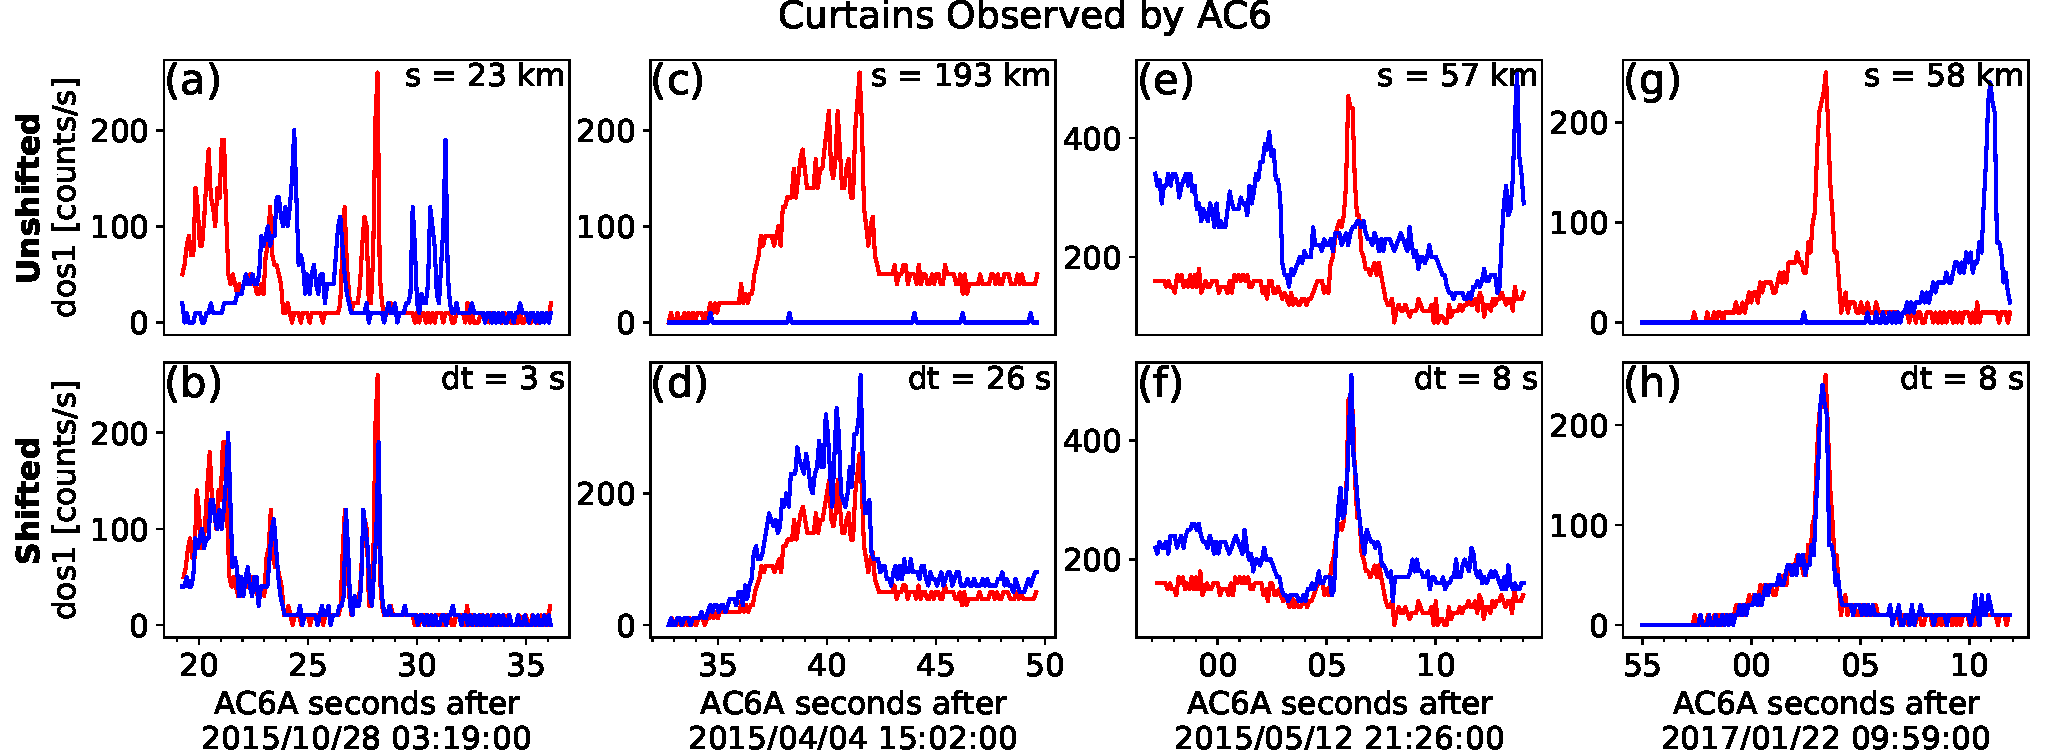
\includegraphics[width=\textwidth]{fig1.pdf}
\caption{Four examples showing the AC6 $> 30$ keV electron data taken by AC6 at the same time in the top row and at the same position in the bottom row. To show the data at the same position the time series data from one spacecraft was shifted by the in-track lag and annotated by dt. These examples show curtain precipitation that was highly correlated for up to 26 seconds.}
\label{fig1}
\end{figure}

\section{Results} \label{results}
\textcolor{blue}{
Outline
\begin{enumerate}
\item Show curtain width and comment how narrow they are. Whether they are drifting or locally precipitating, they must have a very filamentary structure that persists for multiple seconds
\item Figure out how the detection bias affects the width distribution
\item Show, and comment on the Auroral electroject strengths when each curtain was observed. Curtains are more likeliy to be observed during disturbed times.
\item Discuss the SAA, BLC, and show the curtains the the BLC plot. Mention how these electrons must have been precipitating for multiple seconds, over an order of magnitude longer than typical microbursts.
\end{enumerate}
}

In the spirit of brevity, we limited the scope of these results to answer the following three questions:

\begin{enumerate}
\item how narrow are curtains,
\item when and where are curtains observed, and
\item are curtains drifting or locally precipitating?
\end{enumerate}

\begin{figure}
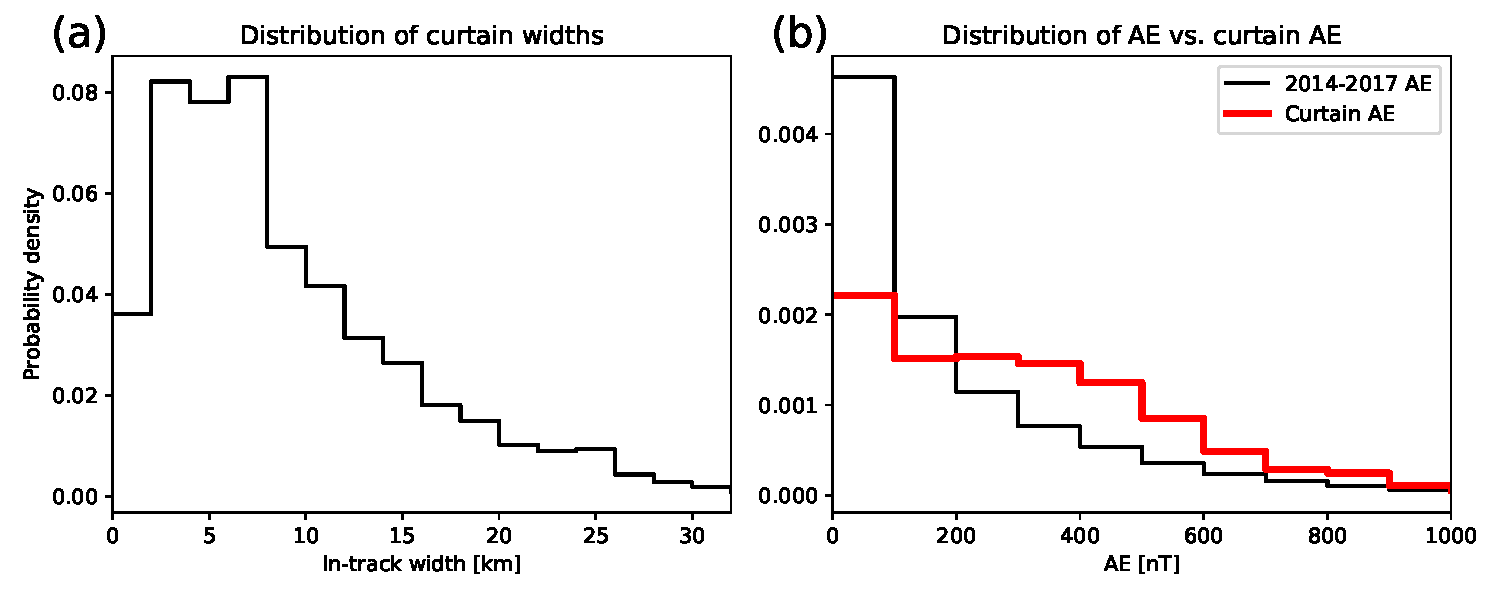
\includegraphics[width=\textwidth]{ac6_curtains_ae_width_dist.pdf}
\caption{Distribution of curtain in-track width (AC6 in-track separation mostly in latitude) in panel a. Panel b shows the distribution of the Auroral Electroject (AE) index from 2014 to 2017 in black, and the AE index when curtains were observed by the thicker red curve.}
\label{ae_width_dist}
\end{figure}

\begin{figure}
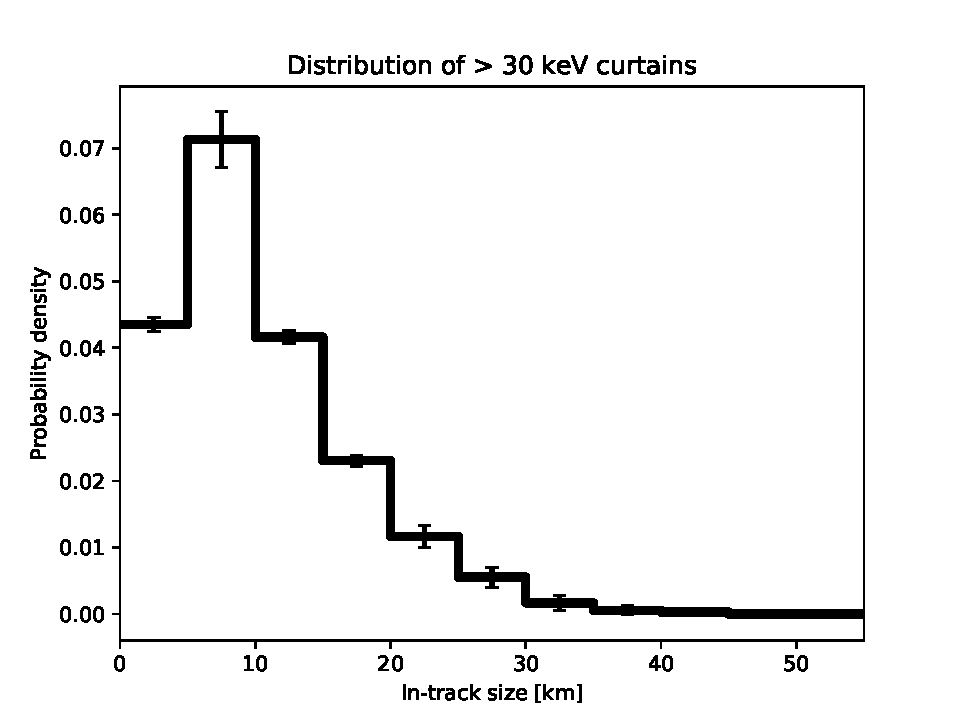
\includegraphics[width=\textwidth]{fig2.pdf}
\caption{Distribution of curtains as a function of L and MLT. To avoid noisy normalization scaling, bins with less than $10,000$ 10 Hz samples were not normalized in panel b. \textcolor{red}{Check that there is no bug interpolating MLT between 24 and 0 hours.}}
\label{fig2}
\end{figure}

\begin{figure}
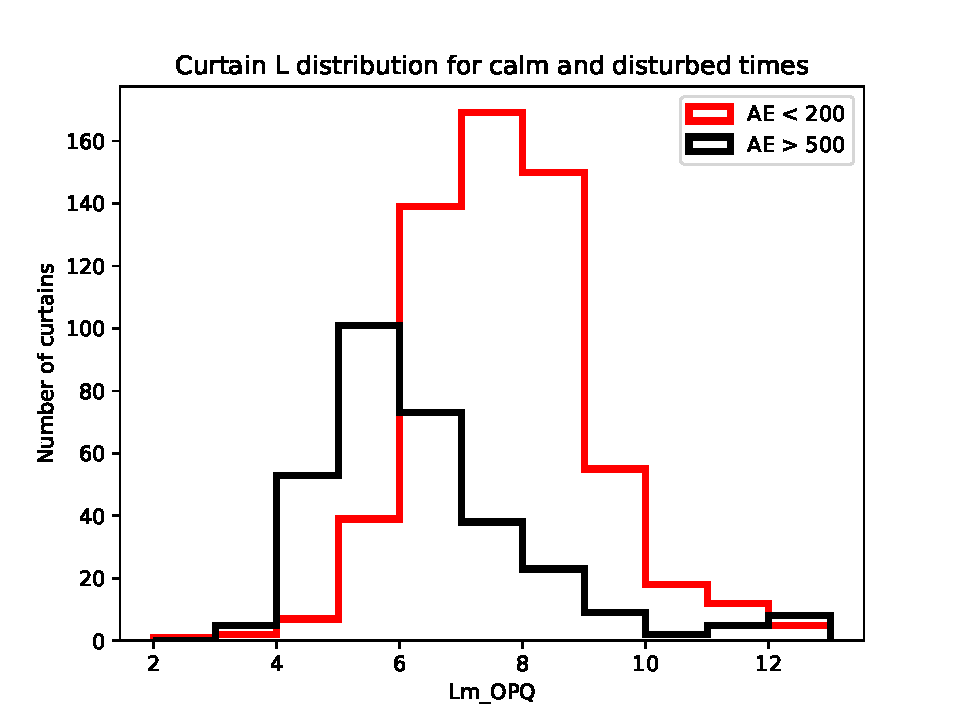
\includegraphics[width=\textwidth]{curtain_L_vs_AE.pdf}
\caption{\textcolor{red}{Or show this figure?}}
\end{figure}

\subsection{Local Atmospheric Precipitation}
\begin{figure}
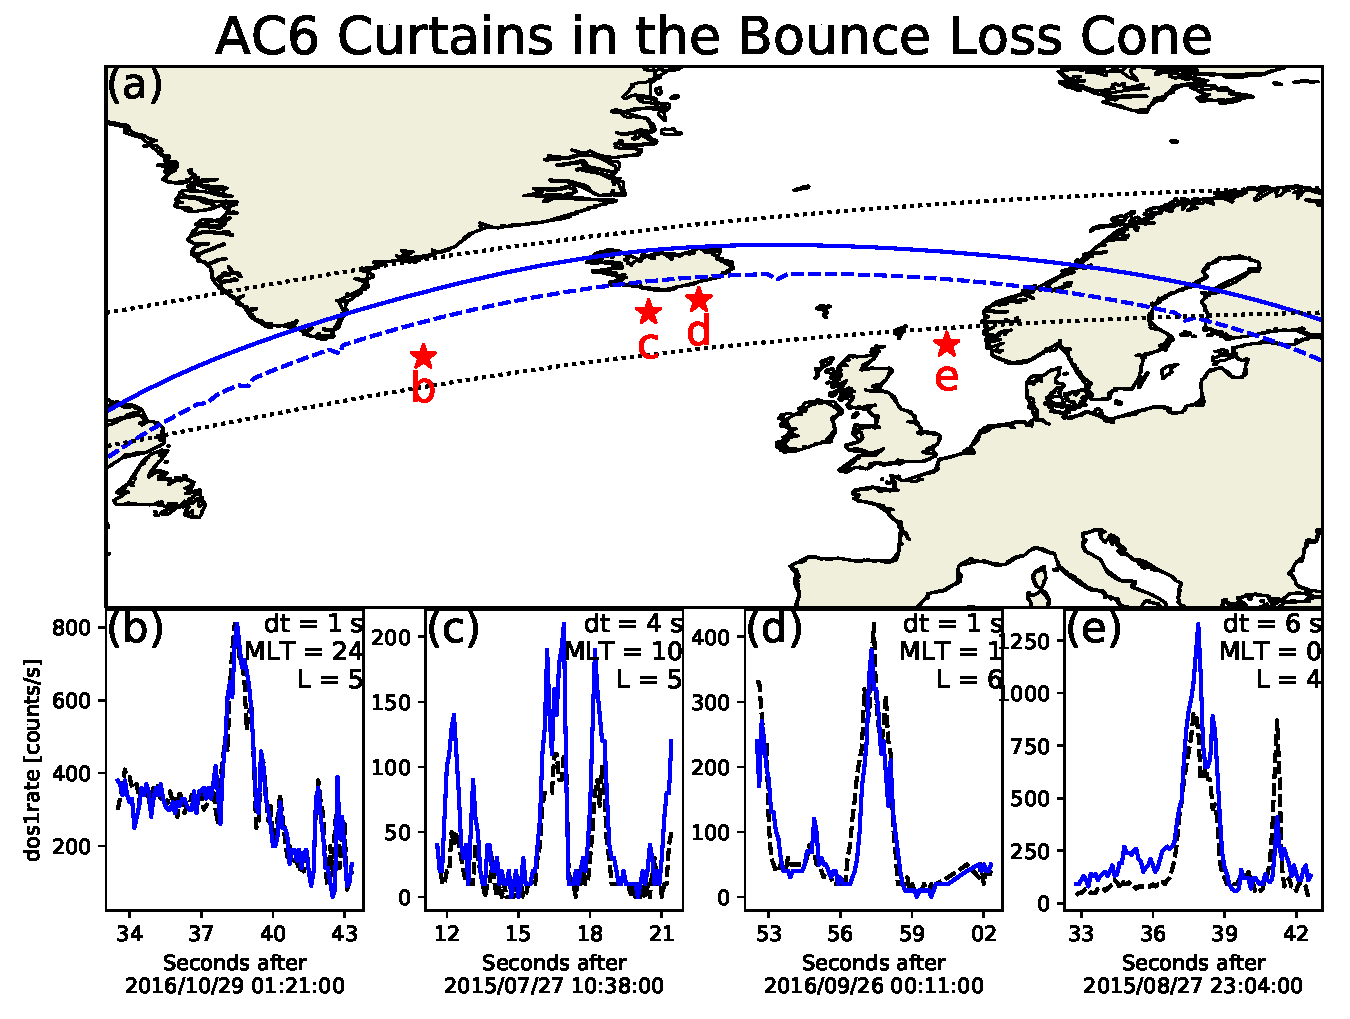
\includegraphics[width=\textwidth]{fig3.pdf}
\caption{Curtains observed inside the bounce loss cone.}
\label{fig3}
\end{figure}

\section{Discussion} \label{discussion}
\textcolor{blue}{
Outline
\begin{enumerate}
\item Curtains are spatially small and must be around a few hundred km at the equator
\item curtain phenomena originates in the outer radiation belt, and observed relatively more in the evening than morning regions. Limited AC6 coverage prevents a complete MLT distribution
\item preference to disturbed conditions
\item some curtains locally precipitate for an extended period of time so there must be a sustained parallel electric field. Show the derivation and estimated potential.
\item AC6 can't answer this question, but curtains could provide a substantial source of HOx and NOX molecules responsible for destroying ozone. We need AC6 with energy and pitch angle resolution.
\end{enumerate}}

\section{Conclusions}

% \appendix

\acknowledgments
This work was made possible with the help from the many engineers and scientists at The Aerospace Corporation who designed, built, and operated AC6. M. Shumko was supported by NASA Headquarters under the NASA Earth and Space Science Fellowship Program - Grant 80NSSC18K1204. D.L. Turner is thankful for support from the Van Allen Probes mission and a NASA grant (Prime award number: 80NSSC19K0280). The work at The Aerospace Corporation was supported in part by RBSP-ECT funding provided by JHU/APL contract 967399 under NASA's Prime contract NAS501072. The AC6 data is available at http://rbspgway.jhuapl.edu/ac6 and the IRBEM-Lib version used for this analysis can be downloaded from https://sourceforge.net/p/irbem/code/616/tree/.

\section{Homeless Words}

Title: Statistical Properties of Curtains--Latitudinally-Narrow and Persistent Electron Precipitation Phenomena

This study leverages AC6, a multi-spacecraft mission, to interpret and understand particle precipitation in a way that is impossible with a single spacecraft.

This study leverages the asymmetry in Earth's magnetic field. The asymmetric magnetic field results in the SAA and the BLC, two very related and unique regions

Particles that impact the atmosphere are lost during that bounce motion. We found curtains in the bounce loss cone, a region in the North Atlantic near and above Iceland.

The bounce loss cone is magnetically connected to the SAA, where Earth's magnetic field is weakest near Earth's surface. A particle observed in the blc in the northern hemisphere will descend below 100 km altitude. At sub-100 km altitudes the particle has a high chance of encountering and scattering with the atmosphere and be lost. 

We found curtain electrons that, when given the chance to execute their cyclical bounce motion, will descend below Earth's surface in the SAA. An electrons can not survive that trip.

Write the paper and ask the question: "What is this paper really about?" Not just curtains, but uncovering something unexpected that has been observed and overlooked for decades.

Are curtains related to aurora? This is a good question---one that is not pertinent here (idea from The Elements of Style p.68).

Here are two parting questions to consider that are not considered here. Why were some curtains shifted slightly? Perhaps it was due to the movement of the magnetic field lines. Also do curtains have a corresponding visual signature on the ground? The answer to this question will show if curtains are related to the aurora.

\bibliography{/home/mike/Dropbox/0_firebird_research/A_presentations/refs}
\bibliography{"refs"}

\end{document}